% Drawing 8/02-2 -- folder 8, batch 02, archive page 29 (PDF page 30).
% Transcription: à droite, un croquis : deux ouverts $U_1$, $U_2$ traversés par une sous-variété (trait épais) le long de laquelle sont $V_1$, $V_2$ ; $\sigma_1$, $\sigma_2$ les envoient dans $\mathbb{R}^m$, où $\sigma_1(V_1)$ et $\sigma_2(V_2)$ sont posés sur $\mathbb{R}^n$
% Kind: two charts U1, U2 along a submanifold, sent by sigma1, sigma2 to R^m. Method 2 (schematic redraw from the facsimile). Status: ok.
% Notes: Two open sets U_1 and U_2 (circles) crossed by a submanifold (thick curve) along which lie V_1 and V_2 (smaller circles); sigma_1 and sigma_2 send them down into R^m, drawn twice: on the left an axis with sigma_1(V_1) set on R^n, on the right sigma_2(V_2) on R^n. The small labels inside the lower ovals are left out.
% Coordinates: 1 unit = 1 mm = 1/100 of the crop width (bbox in page fractions: [0.58, 0.52, 0.98, 0.82]).
% Redrawn by Claude (claude-opus-5-5), issue #73, 2026-11-07; not checked by a human; not compiled (no TeX in the session).
% Rights: reproduces part of the work -- behind RENDER_TRANSCRIPTS, never published by itself.
\documentclass[tikz,border=3pt]{standalone}
\usepackage{amsmath,amssymb}
\usetikzlibrary{patterns,arrows.meta}
\tikzset{pencil/.style={black!45}, struck/.style={black!35}, mark/.style={circle,draw,inner sep=1.3pt}, pt/.style={circle,fill,inner sep=0.9pt}, opt/.style={circle,draw,fill=white,inner sep=1.1pt}}
\begin{document}
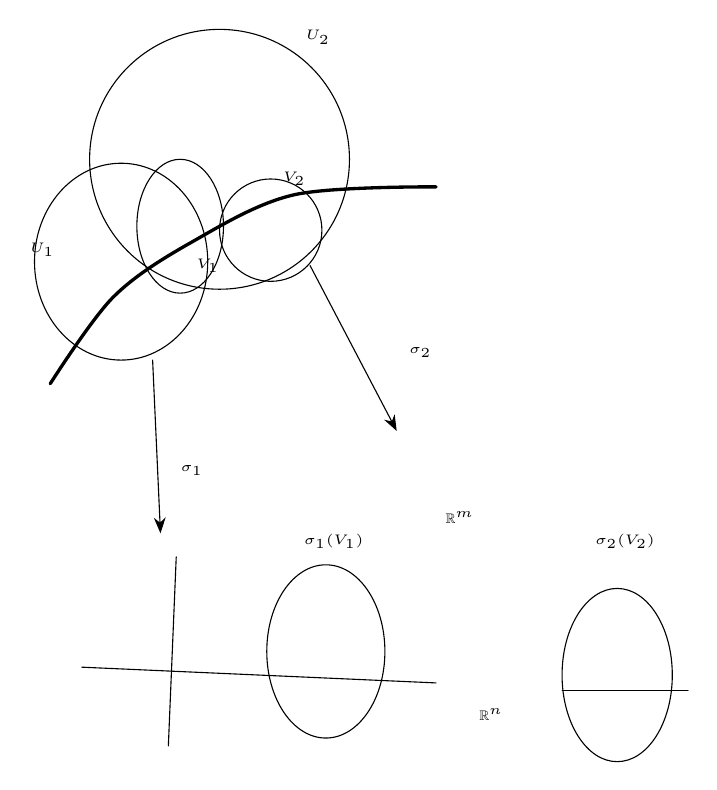
\begin{tikzpicture}[x=1mm,y=1mm,line cap=round,line join=round,font=\scriptsize]
\draw (22,-37.5) ellipse[x radius=11, y radius=12.5];
\draw (34.5,-24.5) ellipse[x radius=16.5, y radius=16.5];
\draw (29.5,-33) ellipse[x radius=5.5, y radius=8.5];
\draw (41,-33.5) ellipse[x radius=6.5, y radius=6.5];
\draw[very thick] plot[smooth, tension=0.55] coordinates {(13,-53) (21,-42) (31,-35) (44,-29) (62,-28)};
\node[inner sep=1pt] at (12,-36) {\tiny $U_1$};
\node[inner sep=1pt] at (47,-9) {\tiny $U_2$};
\node[inner sep=1pt] at (33,-38) {\tiny $V_1$};
\node[inner sep=1pt] at (44,-27) {\tiny $V_2$};
\draw[-{Stealth[length=2mm]}] (26,-50) -- (27,-72);
\node[inner sep=1pt] at (31,-64) {\tiny $\sigma_1$};
\draw[-{Stealth[length=2mm]}] (46,-38) -- (57,-59);
\node[inner sep=1pt] at (60,-49) {\tiny $\sigma_2$};
\node[inner sep=1pt] at (65,-70) {\tiny $\mathbb{R}^m$};
\draw (29,-75) -- (28,-99);
\draw (17,-89) -- (62,-91);
\draw (48,-87) ellipse[x radius=7.5, y radius=11];
\node[inner sep=1pt] at (49,-73) {\tiny $\sigma_1(V_1)$};
\node[inner sep=1pt] at (69,-95) {\tiny $\mathbb{R}^n$};
\draw (78,-92) -- (94,-92);
\draw (85,-90) ellipse[x radius=7, y radius=11];
\node[inner sep=1pt] at (86,-73) {\tiny $\sigma_2(V_2)$};
\end{tikzpicture}
\end{document}
